\chapter{Représentation d'état, commandabilité, observabilité}
\section{Représentation d'état}
\subsubsection{Cas des systèmes continus}
\footnote{Il n'y a pas unicité de la représentation d'état}
\footnote{Les matrices A,B, C, D sont à coefficient constants}
\LARGE{
    \[
\left \{
\begin{array}{c @{=} c}
    \dot x(t) & f(x(t),u(t),t)\\
    y(t) & g(x(t),u(t),t)
\end{array}
\right.
\] 
} 
\label{RepEtat_Continu}
\newline
\large{
Avec : $x \in R^{n}, y \in R^{p}, u \in R^{p}$
}
\subsubsection{Cas des SLCI}
\LARGE{
    \[
\left \{
\begin{array}{c @{=} c}
    \dot x(t) & Ax(t) + Bu(t)\\
    y(t) & Cx(t) + Du(t)
\end{array}
\right.
\]
}
\begin{equation}
    \Large{\hbox{}}
    \label{RepEtat_SLCI}
\end{equation}
\newpage
\begin{itemize}
    \item \textcolor{BrickRed}{A : matrice d'évolution $dim(A) = n^{2}$ (matrice carrée)}
    \item \textcolor{BrickRed}{B : matrice d'entrée $dim(B) = n$ (vecteur colonne)}
    \item \textcolor{BrickRed}{C : matrice de sortie $dim(C) = m$ (vecteur ligne)}
    \item \textcolor{BrickRed}{D : matrice ?? de transmission directe $D \in \mathbb{R}$ (réel)}
\end{itemize}
\subsubsection{Cas des systèmes discrets}
\LARGE{
    \[
\left \{
\begin{array}{c @{=} c}
    x[k+1] & f(x[k],u[k],k)\\
    y[k] & g(x[k],u[k],k)
\end{array}
\right.
\]
} 
\label{RepEtat_Discret}
\newline
Avec : $x \in R^{n}, y \in R^{p}, u \in R^{p}$
\subsubsection{Cas des SLDI}
\LARGE{
    \[
\left \{
\begin{array}{c @{=} c}
    x[k+1] & Fx[k] + Gu[k]\\
    y[k] & Cx[k] + Du[k]
\end{array}
\right.
\]
}
\begin{equation}
    \label{RepEtat_SLDI}
\end{equation}
\newpage
\section{Point d'équilibre}
On dit que le triplet $(\overline{x},\overline{u},\overline{y})$ est un point d'équilibre SSI, il vérifie la condition suivante :
\subsubsection{En continu} 
$\forall t \in R$
\begin{center}
    \LARGE{
    \[
\left \{
\begin{array}{c @{=} c}
    0 & f(\overline{x},\overline{u}, t)\\
    \overline{y} & g(\overline{x},\overline{u},t)
\end{array}
\right.
\]  
}
\end{center}
Avec : $\frac{dx(t_{eq})}{dt} = \frac{d\overline{x}}{dt} = 0$
\subsubsection{En discret}
$\forall k \in N,$
\begin{center}
    \LARGE{
    \[
\left \{
\begin{array}{c @{=} c}
    \overline{x} & f(\overline{x},\overline{u},k)\\
    \overline{y} & g(\overline{x},\overline{u},k)
\end{array}
\right.
\]
}
\end{center}
Avec : $x[k+1] - x[k] = 0$
\newline
\section{Solution de la représentation d'état}
\subsection{Cas des SLCI}
La représentation d'état des SLCI \eqref{RepEtat_SLCI} mène à la solution suivante : 
\begin{center}
    \Large{$
    x(t) = e^{A(t-t_{0})}x(t_{0}) + 
     \int_{t}^{t_{0}}{ e^{A(t-t_{0})Bu(\tau)} \,d\tau}
    $} 
    \footnote{
    En considérant $e^{At}$ comme une combinaison linéaire de $I_{n}$ et les $(A^{i})_{i \in N}$ tel que : \newline
    $e^{At} = \sum_{i=0}^{\infty}{
    \frac{A^{i}t^{i}}{i!} = 
    I_{n} + At + A^{2}\frac{t^{2}}{2!} + ...
    }$
    }
\end{center}

\subsection{Cas discret}
La représentation d'état des SLDI \eqref{RepEtat_SLDI} mène à la solution suivante : 
\begin{center}
    \Large{$
    x[k] = F^{k-k_{0}}x[k_{0}] + 
    \sum_{j=k_{0}}^{k-1}{F^{k-j-1}Gu[j]}
    $} 
    \footnote{Raisonnement par récurrence en conjecturant l'expression de $x[k]$ à partir de \eqref{RepEtat_SLDI}: \newline
    $x[k] = Fx[k-1] + Gu[k-1]$ \newline
    $x[k] = F^{2}x[k-2] + FGu[k-2] + Gu[k-1]$ \newline
    $x[k] = F^{3}x[k-3] + F^{2}Gu[k-3] +  FGu[k-2] + Gu[k-1]$ \newline
    ... \newline
    $x[k] = F^{k-k_{0}}x[k_{0}] + 
    \sum_{j=k_{0}}^{k-1}{F^{k-j-1}Gu[j]}$
    }
\end{center}
Avec : \newline

\Large{
$F = e^{AT_{e}}$ \newline

$G = \int_{0}^{T_{e}}{ e^{A\theta}B \,d\theta}$
}
\newpage
\section{Représentation de la stabilité}
\begin{center}
    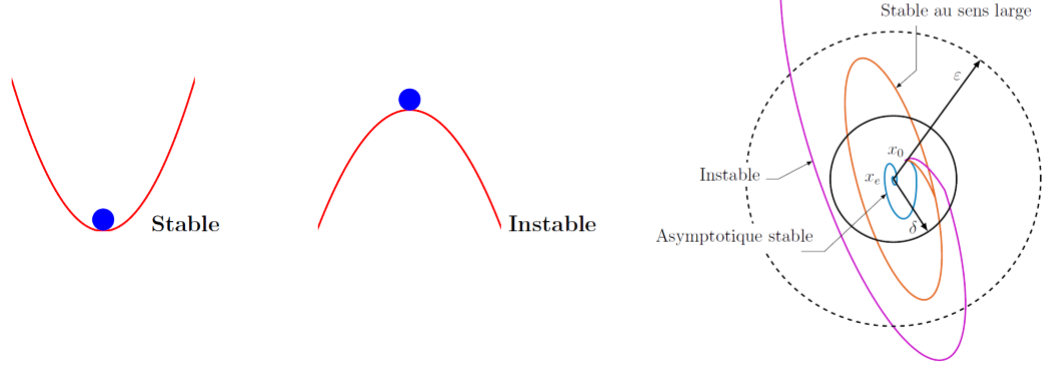
\includegraphics[scale=0.6]{Pics/Stabilite.png}
\end{center}
\section{Modélisation de la stabilité}
\subsection{Stabilité au sens de Lyapunov}
$\overline{x}$ est stable au sens de Lyapunov SSI :
\begin{center}
    \Large{$
    \forall \epsilon > 0, \forall t_{0}, \exists \delta(\epsilon, t_{0}), \newline
    \left\lvert\lvert \overline{x} - x(t_{0}) \right\rvert\rvert < \delta(\epsilon,t_{0}) 
    \implies \left\lvert\lvert x(t) - \overline{x} \right\rvert\rvert < \epsilon, \forall t t_{0}
    $}
\end{center}
\subsection{Stabilité asymptotique}
$\overline{x}$ est stable asymptotiquement SSI :
\begin{center}
    \Large{$
    \exists \delta_{1}(t_{0}), \left\lvert\lvert \overline{x} - x(t_{0}) \right\rvert\rvert < \delta_{1}t_{0} \implies
    \lim_{t \to \infty}{\left\lvert\lvert x(t) - \overline{x} \right\rvert\rvert} = 0
    $}
\end{center}
\subsection{Stabilité exponentielle}
$\overline{x}$ est exponentiellement stable SSI
\begin{itemize}
    \item $\overline{x}$ est assymptotiquement stable
    \item \Large{$
            \exists M 0 ,\exists \alpha 0, \forall t > t_{0} \newline
            \left\lvert\lvert \overline{x} - x(t_{0}) \right\rvert\rvert < 
            M \left\lvert\lvert \overline{x} - x(t) \right\rvert\rvert e^{-\alpha(t-t_{0})} 
            $}
\end{itemize}
\newpage
\begin{itemize}
    \item Pour un système \textbf{continu} tel que :
    \Large{
        \[
    \left \{
    \begin{array}{c @{=} c}
        \dot x(t) & Ax(t) + Bu(t)\\
        y(t) & Cx(t) + Du(t)
    \end{array}
    \right.
    \]
    }
    \Large{le système est dit \textbf{stable} SSI $\forall \lambda \in Sp(A)$\footnote{$\lambda$ valeur propre de $A$}, on a} \newline
    \begin{center}
        \Large{\fbox{$Re(\lambda) < 0$}}\footnote{\textbf{\textcolor{BrickRed}{Critère de Routh}}} \newline
    \end{center}
    \large{$\forall \lambda \in Sp(A)$ tel que $Re(\lambda) = 0$, les $\lambda$ ont une multiplicité algébrique (géométrique)}

    \item \Large{Pour un système \textbf{discret} tel que :}
    \Large{
        \[
    \left \{
    \begin{array}{c @{=} c}
        x[k+1] & Fx[k] + Gu[k]\\
        y[k] & Cx[k] + Du[k]
    \end{array}
    \right.
    \]
    }
    \Large{le système est dit \textbf{stable} SSI $\forall \lambda \in Sp(F)$\footnote{$\lambda$ valeur propre de $F$}, on a} \newline
    \begin{center}
        \Large{\fbox{$\left\lvert \lambda \right\rvert < 1$}}\footnote{\textbf{\textcolor{BrickRed}{Critère de Jury}}} \newline
    \end{center} 
    \large{$\forall \lambda \in Sp(F)$ tel que $Re(\lambda) = 1$, les $\lambda$ ont une multiplicité algébrique (géométrique)}    
\end{itemize}
\footnote{Dans les deux cas, les sytèmes qui vérifient ces conditions sont dit stables \textbf{assymptotiquement} \textbf{exponentiellement}}
\newpage
\subsection{Stabilité Entrée Bornée Sortie Bornée (EBSB)}
\subsubsection{\Large{cas continu}}
Soit $h$ la fonction de transfert du système définit par \eqref{RepEtat_SLCI}. Ce système est dit de stabilité EBSB SSI : \newline
\begin{center}
    \Large{\fbox{$
    \int_{-\infty}^{+\infty}{ |h(t)| \,dt} < +\infty
    $}}
\end{center}
un système causal de fonction de transfert $H$ est dit de stabilité EBSB SSI \textbf{tous les pôles de la fonction $H(p)$ ont une partie réelle strictement négative (critère de Routh)}
\subsubsection{\Large{cas discret}}
Soit $h$ la fonction de transfert du système définit par \eqref{RepEtat_SLDI}. Ce système est dit de stabilité EBSB SSI : \newline
\begin{center}
    \Large{\fbox{$
    \sum_{-\infty}^{+\infty}{ |h[k]| \,dk} < +\infty
    $}}
\end{center}
un système causal de fonction de transfert $H$ est dit de stabilité EBSB SSI \textbf{tous les pôles de la fonction $H(z)$ ont un module strictement inférieur à 1 (critère de Jury)}
\newpage
\section{Passage de la représentation d'état à la fonction de transfert}
\subsubsection{Cas continu}
\LARGE{
    \[
\left \{
\begin{array}{c @{=} c}
    \dot x(t) & Ax(t) + Bu(t)\\
    y(t) & Cx(t) + Du(t)
\end{array}
\right.
\]
$\implies$ \Large{\fbox{$
H(s) = C[sI_{n} - A]^{-1}B + D
$}}
\subsubsection{Cas discret}
\LARGE{
    \[
\left \{
\begin{array}{c @{=} c}
    x[k+1] & Fx[k] + Gu[k]\\
    y[k] & Cx[k] + Du[k]
\end{array}
\right.
\]
$\implies$ \Large{\fbox{$
H(z) = C[sI_{n} - F]^{-1}G + D
$}}
\section{Passage de la fonction de transfert à la représentation d'état}
Soit une fonction de transfert de la forme : \newline
\begin{center}
    \LARGE{$
    H(p) = \frac{\sum_{i=0}^{m} b_{i}(p)p^{i}}{\sum_{j=0}^{n} a_{j}(p)p^{j}} =
            \frac{b_{0} + b_{1}p + ... + b_{m}p^{m}}{a_{0} + a_{1}p + ... + a_{n-1}p^{n-1} + p^{n}}
    $}
\end{center}
\newpage
\begin{itemize}
    \item Si $m < n \implies D = 0$ \newline
        \[A =
        \begin{bmatrix}
            0 & 1 & 0 & 0 & 0 \\
            0 & 0 & 1 & 0  & 0 \\
            \vdots & \vdots & \vdots & \ddots & \vdots \\
            0 & 0 & 0 & 0 & 1 \\
            -a_{0} & -a_{1} & -a_{2} & \dots  & -a_{n-1}
        \end{bmatrix}
        ,B = 
        \begin{bmatrix}
            0 \\
            0 \\
            \vdots \\
            0 \\
            1
        \end{bmatrix}
        \]    
        \[C = 
        \begin{bmatrix}
            b_{0} & b_{1} & ... & b_{m} & 0 & .. & 0
        \end{bmatrix}
        \] \newline
    \item Si $m = n \implies D = b_{n}$
        et on cherche $\tilde{H(p)}$ tel que : \newline
        
        $H(p) = \tilde{H(p)} + D$ \newline
\end{itemize}
Soit une fonction de transfert de la forme : \newline
\begin{center}
    \LARGE{$
    H(p) = \frac{\sum_{i=0}^{n-1} b_{i}(p)p^{i}}{\sum_{j=0}^{n} a_{j}(p)p^{j}} =
            \frac{b_{0} + b_{1}p + ... + b_{n-1}p^{n-1}}{a_{0} + a_{1}p + ... + a_{n-1}p^{n-1} + p^{n}}
    $}
\end{center}
Alors : \newline
\[A = 
\begin{bmatrix}
    0 & 0 & 0 & 0 & -a_{0} \\
    1 & 0 & 0 & 0  & -a_{1} \\
    \vdots & \vdots & \vdots & \ddots & \vdots \\
    0 & 0 & 0 & 0 & 1 \\
    0 & \vdots & 0 & 1 & -a_{n-1}
\end{bmatrix}
,B = 
\begin{bmatrix}
    b_{0} \\
    b_{1} \\
    \vdots \\
    b_{n-2} \\
    b_{n-1}
\end{bmatrix}
\]    
\[C = 
\begin{bmatrix}
    b_{0} & b_{1} & ... & b_{m} & 0 & .. & 0
\end{bmatrix}
\] 
\newpage
\section{Changement de base}
\subsubsection{Cas continu}
\LARGE{
    \[
\left \{
\begin{array}{c @{=} c}
    \dot x(t) & Ax(t) + Bu(t)\\
    y(t) & Cx(t) + Du(t)
\end{array}
\right.
\]
$\Longleftrightarrow$
\Large{
    \[
\left \{
\begin{array}{c @{=} c}
    \dot{\overline{x}}(t) & T^{-1}AT\overline{x}(t) + T^{-1}Bu(t) \\
    y(t) & CT\overline{x}(t) + Du(t)
\end{array}
\right.
\]
\footnote{$\overline{x} = Tx$}
\subsubsection{Cas discret}
\LARGE{
    \[
\left \{
\begin{array}{c @{=} c}
    x[k+1] & Fx[k] + Gu[k]\\
    y[k] & Cx[k] + Du[k]
\end{array}
\right.
\]
$\Longleftrightarrow$
\LARGE{
    \[
\left \{
\begin{array}{c @{=} c}
    x[k+1] & T^{-1}FTx[k] + T^{-1}Gu[k]\\
    y[k] & CTx[k] + Du[k]
\end{array}
\right.
\]
\newpage
\section{commandabilité - systèmes commandables}
\large{Un système est dit commandable si :}
\begin{itemize}
    \item $\exists u(t)$ ou $\exists u[k]$ qui permet de passer de l'état \textbf{quelconque $x_{0}$ à $x_{1}$ quelconque} en un temps fini.
    \item \textbf{\large{Critère de Kalman : }}
        \subsubsection{Cas continu}
        \large{Soit la \textbf{matrice de commandabilité $Q_{c}$ :}}
            \[
            Q_{c} =
            \begin{bmatrix}
                B & AB & A^{2}B & ... & A^{n-1}B
            \end{bmatrix}
            \in M_{n,n}(C)
            \]
        \begin{center}
            \fbox{\Large{$rg(Q_{c}) = n$}}\footnote{$n$ colonnes indépendantes. La matrice $Q_{c}$ est formée par les vecteurs $(A^{i}B)_{i \in \mathbb{N}}$ avec A une matrice carrée de taille n et B un vecteur colonne de taille n}
        \end{center}
        \subsubsection{Cas discret}
        \large{Soit la \textbf{matrice de commandabilité $Q_{c}$ :}}
        \[
        Q_{c} =
        \begin{bmatrix}
            G & FG & F^{2}G & ... & F^{n-1}G
        \end{bmatrix}
        \in M_{n,n}(C)
        \]
        \begin{center}
            \fbox{\Large{$rg(Q_{c}) = n$}}
        \end{center}
    \item  \textbf{\large{Critère de Popov-Belevich-Hautus}}
        \subsubsection{Cas continu}
        \begin{center}
            \[
                \forall p \in \mathbb{C}, 
                rg(
                \begin{bmatrix}
                    pI_{n} - A & B
                \end{bmatrix}
                ) = n
            \]
        \end{center}
        \subsubsection{Cas discret}
        \begin{center}
            \[
                \forall z \in \mathbb{C}, 
                rg(
                \begin{bmatrix}
                    zI_{n} - F & G
                \end{bmatrix}
                ) = n
            \]
        \end{center}
\end{itemize}
\newpage
\section{commandabilité - systèmes partiellement commandables}
\begin{itemize}
    \item Un système est dit partiellement commandable SII $rg(Q_{c}) \inf n, \forall x(t_{0}) = 0$, l'état $x(t)$ ou $x[k]$ reste dans le sous-espace vectoriel E tel que $dim(E) = q$ engendré par $Q_{c}$
    \item Il existe une base de l'espace d'état permettant de séparer l'état en partie commandable et la partie non commandable
\end{itemize}
\section{Interprétation de la commandabilité}
\textbf{\textcolor{BrickRed}{Théorème de Wonham : }} \newline
Pour un système commandable, la commande par retour d'état permet de placer les pôles de la fonction de transfert arbitrairement 
\newpage
\section{observabilité}
\begin{itemize}
    \item \large{Un système est dit totalement observable SII pour un \textbf{état quelconque $x_{0}$}, l'observation de $y(t)$ ou de $y[k]$ sur une durée finie permet de déterminer $x_{0}$\footnote{Sinon, le système est dit \textbf{partiellement observable}}}
    \item \textbf{Critère de Kalman}
        \subsubsection{Cas continu}
        Soit
        \[ Q_{c} = 
        \begin{bmatrix}
            C \\
            CA \\
            ... \\
            CA^{n-1}
        \end{bmatrix}
        \in M_{n}(\mathbb{C})
        \]
        \begin{center}
            \fbox{\Large{$rg(Q_{0}) = n$}} \footnote{$n$ lignes indépendantes. La matrice $Q_{0}$ est formée par les vecteurs ligne $(CA^{i})_{i \in \{1,n-1 \}}$ avec $A$ matrice carrée de taille $n$ et $C$ vecteur ligne de taille $n$}
        \end{center}
        \subsubsection{Cas discret}
        \[
        Q_{0} =
        \begin{bmatrix}
            C \\
            CF \\
            ... \\
            CF^{n-1}
        \end{bmatrix} 
        \in M_{n}(\mathbb{C})
        \]
        \begin{center}
            \fbox{\Large{$rg(Q_{0}) = n$}}
        \end{center}
        \newpage
    \item \textbf{Critère de Popov-Belevich-Hautus}
        \subsubsection{Cas continu}
        \begin{center}
            \[
            rg(
                \begin{bmatrix}
                    pI_{n} - A \\
                    C
                \end{bmatrix}
            ) = n
            \] 
        \end{center}
        \footnote{$\forall p \in \mathbb{C}$}
        \subsubsection{Cas discret}
        \begin{center}
            \[
            rg(
                \begin{bmatrix}
                    zI_{n} - A \\
                    C
                \end{bmatrix}
            ) = n
            \]
        \end{center}
        \footnote{$\forall z \in \mathbb{C}$}
\end{itemize}
\newpage
\section{Forme canonique de Kalman}
Soit un système représenté par :
\large{
    \[
\left \{
\begin{array}{c @{=} c}
    \dot x(t) & Ax(t) + Bu(t)\\
    y(t) & Cx(t) + Du(t)
\end{array}
\right.
\]
$\exists$ un transformation 
\[ \tilde{x}(t) =
\begin{bmatrix}
    \tilde{x}_{co} \\
    \tilde{x}_{c\tilde{o}} \\
    \tilde{x}_{\tilde{c}\tilde{o}} \\
    \tilde{x}_{\tilde{c}o} 
\end{bmatrix}
= Tx(t)\]
$T$ inversible tel que : \newline
\large{
    \[
\left \{
\begin{array}{c @{=} c}
    \dot \tilde{x}(t) & \tilde{A}\tilde{x(t)} + \tilde{B}u(t)\\
    y(t) & \tilde{C}\tilde{x}(t) + Du(t)
\end{array}
\right.
\]
Avec :
\begin{itemize}
    \item $ ( 
        \begin{bmatrix}
            \tilde{A}_{co} & 0 \\
            \tilde{A}_{21} & \tilde{A}_{c \tilde{o}}  
        \end{bmatrix}
        ,
        \begin{bmatrix}
            \tilde{B}_{co} \\
            \tilde{B}_{c\tilde{o}}
        \end{bmatrix}
    )$ commandable \newline
    \item $ ( 
        \begin{bmatrix}
            \tilde{A}_{co} & \tilde{A}_{13} \\
            0 & \tilde{A}_{\tilde{c} o}  
        \end{bmatrix}
        ,
        \begin{bmatrix}
            \tilde{C}_{co} & \tilde{C}_{\tilde{c} o}
        \end{bmatrix}
    )$ observable \newline
    \item $
    H(p) = C(pT_{n} - A)^{-1}B + D = \tilde{C_{co}}(pI_{n} - \tilde{A}_{co})^{-1}\tilde{B}_{co} + D
    $
\end{itemize}
\[\tilde{A} = 
    \begin{bmatrix}
        \tilde{A}_{co}  & 0                         & \tilde{A}_{13}          & 0\\
        \tilde{A}_{21}  & \tilde{A}_{c\tilde{o}}    & \tilde{A}_{23}          & \tilde{A}_{24}  \\
        0               & 0                         & \tilde{A}_{\tilde{c} o} & 0 \\
        0               & 0                         & \tilde{A}_{43}          & \tilde{A}_{\tilde{c}\tilde{o}} \\
    \end{bmatrix}
    \] \newline
\[\tilde{B} = 
    \begin{bmatrix}
        \tilde{B}_{co} \\
        \tilde{B}_{c\tilde{o}} \\
        0 \\
        0 \\
    \end{bmatrix}
    \]
\[\tilde{C} = 
    \begin{bmatrix}
        \tilde{C}_{co} & 0 & \tilde{C}_{\tilde{c} o } & 0
    \end{bmatrix}
    \]